\documentclass[12pt,a4paper]{article}

% Packages
\usepackage[utf8]{inputenc}
\usepackage{graphicx}
\usepackage{amsmath}
\usepackage{amssymb}
\usepackage{hyperref}
\usepackage{geometry}
\usepackage{titlesec}
\usepackage{fancyhdr}
\usepackage{enumitem}
\usepackage{booktabs}
\usepackage{xcolor}
\usepackage{float}
\usepackage{natbib}

% Page layout
\geometry{a4paper, margin=1in}
\pagestyle{fancy}
\fancyhf{}
\rhead{\thepage}
\rhead{\thepage}
\lhead{\leftmark}

% Title formatting
\titleformat{\section}{\Large\bfseries}{\thesection}{1em}{}
\titleformat{\subsection}{\large\bfseries}{\thesubsection}{1em}{}

% Colors
\definecolor{titlecolor}{RGB}{0, 51, 102}

% Title page
\title{\color{titlecolor}\Huge GFSL-A GPU Friendly Skiplist}
\author{Deven Anil Gangwani(210327) \and Shivam Sharma(210983)}
\date{\today}

\begin{document}

% Title page
\maketitle
\thispagestyle{empty}
\newpage

% Abstract
\begin{abstract}
    \noindent
    The GPU-friendly skiplist is a probabilistic data structure that uses warp-coalesced operations to reduce memory accesses and divergence between threads. In this presentation, we go over the details of the data structure, including various implementational aspects and insights and performance variations compared to a naive skiplist implementation. We go on to discuss various improvements made to the data structure, their impact, and future work to optimize the data structure further, and particularly for out-of-memory applications.
\end{abstract}

% Table of Contents
\tableofcontents
\newpage

% Main content
\section{Introduction}

\subsection{Background}
GPUs lack a robust set of battle-tested data structures, especially primitive ones, largely because designing
them is inherently difficult due to the GPU's distinct computational model compared to CPUs. Consequently,
CPU-based data structures often don't translate effectively one-to-one onto GPUs. This necessitates
the development of GPU-specific versions explicitly designed to work harmoniously with the GPU computation model,
tackling major challenges like mitigating branch divergence and memory divergence to achieve optimal performance.

\subsection{Cuda Computational Model}
The Nvidia GPU computation model utilizes a Single Instruction, Multiple Threads (SIMT) approach. In this model,
threads running on the same Streaming Multiprocessor (SM) subprocessor execute the identical instruction simultaneously in groups of 32, called "warps." Parallelism is achieved because the data processed by each thread within the warp can vary. While pre-Volta architecture GPUs mandated strict lockstep execution for threads within a warp, this constraint has been eased in Volta and later architectures. Two critical performance considerations are-
\begin{itemize}
    \item Branch Divergence: This occurs when the control flow for two (or more) threads within the same warp is different; for example, if some threads in a warp take the if path of a conditional statement while others take the else path. 
    \item Memory Divergence: This happens when two (or more) threads within the same warp access different global memory locations, which leads to multiple, less efficient memory transactions instead of potentially coalescing them into fewer transactions.
\end{itemize}

\section{Parallel Skiplists}
\subsection{Skiplist Data Structure}
A Skiplist is a probabilistic data structure that provides efficient search, insertion, and deletion operations (averaging O(log n) time), similar to balanced trees, but often simpler to implement.

It uses multiple levels of sorted linked lists. The lowest level contains all elements. Each element has a random probability (e.g., 50\%) of also being included in the next level up. This creates "express lanes" – higher levels skip over multiple elements in the lower levels. Searching starts at the highest level, traverses forward as far as possible without overshooting the target, then drops down to the next level, repeating until the element is found (or determined absent) in the bottom-most list.

\begin{figure}[H]
    \centering
    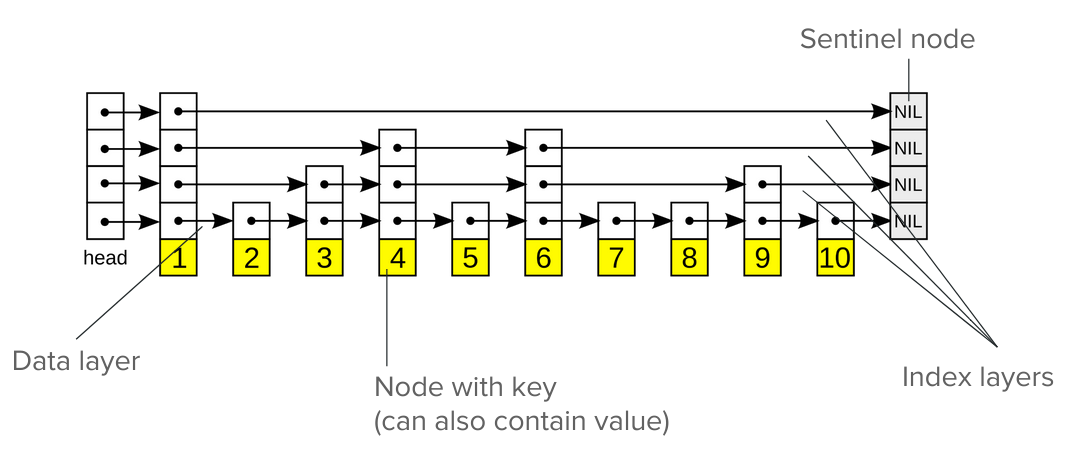
\includegraphics[width=0.8\textwidth]{1.png}
    \caption{An example Skiplist}
\end{figure}



\subsection{Parallel and Lock-Free Skiplists}
Implementing skiplsits in parallel environments requires significant care. The core challenge arises because inserting or deleting a key involves simultaneously modifying nodes across potentially multiple linked lists. If not properly managed, concurrent operations can easily lead to data structure corruption. A straightforward solution to ensure safety is to employ locks on all relevant nodes, similar to techniques used for concurrency-safe standard linked lists. Specifically, during an insertion, the process involves determining the key's maximum height, then locking the predecessor nodes just before the insertion point in each layer, proceeding from the bottom layer upwards; these locks are subsequently released in the reverse order (top-down) after the insertion is complete, but such a scheme in not very scalable and limits concurrency.

Lock-Free Skiplists are a more scalable alternative. They use atomic operations to ensure thread safety, allowing multiple threads to operate on the same data. One such implementation is described in \citep{herlihy2012art}, with the core idea being-

\begin{itemize}
    \item Each layer is a lock-free linked list, so atomic operations used to mutate each layer
    \item Node is considered in the list if present in data layer, may temporarily be in upper layers without being in lowermost layer.
    \item Insertion: first insert the node in the bottom-most linked list, then linked in upper levels.
    \item Deletion: find the node in the lowermost level (and the other levels), mark nodes for removal by node-search function (not the search operation) used by insert and delete from the top level downwards, marking lowermost node in the end.
\end{itemize}

This implementation is ported to CUDA in \citep{mnc}, which would be referred to as M\&C from now on.

\section{GFSL}
The entire GFSL algorithm is described in \citep{gfsl}. With the main points beings laid out here.

\subsection{Design Principles}
GFSL is designed to minimize the warp-divergence and memory-divergence by using warp-coalesced operations by-

\begin{itemize}
    \item A single operation(insert, erase or search) is performed by a warp of threads(32 threads). With the inter thread communication being done through highly efficient inter warp intrinsics, without causing divergence.
    \item A single node in GFSL, called Chunk from now on, consists of 30 KV pairs, a next and max field and a lock field, totalling to 256 bytes. This allows the chunk to be read by a warp in only 2 coalesced memory transactions.
\end{itemize}

\begin{figure}[H]
    \centering
    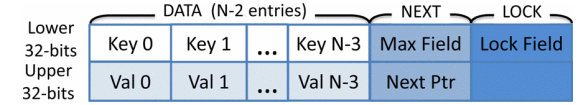
\includegraphics[width=0.8\textwidth]{2.png}
    \caption{Chunk Structure}
\end{figure}

\subsection{GFSL Structure}
GFSL contains a hierarchy of Chunk linked lists(level 0-31). The 0th level is the data layer, which stores the actual KV paris. The layers 1-31 are called index layers, and store pointers to the Chunk in the lower level.

\begin{figure}[H]
    \centering
    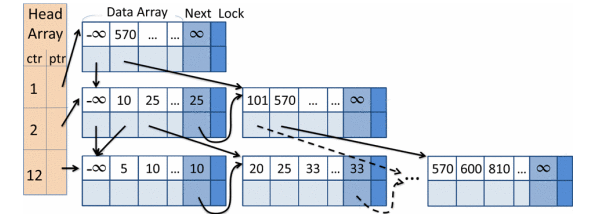
\includegraphics[width=0.8\textwidth]{3.png}
    \caption{GFSL Structure}
\end{figure}

\subsection{Search Operation}
\begin{figure}[H]
    \centering
    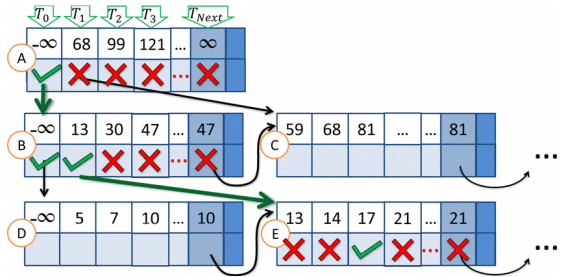
\includegraphics[width=0.6\textwidth]{4.png}
    \caption{A warp searching for key 17}
\end{figure}

The search operation is fairly similar to how search is done in a regular skiplist. The warp starts with the first chunk in the highest occupied index layer and moves forward in the level until it finds the first Chunk whose max field is greater than or equal to the searh key, at this point, the warp steps down to the lower level through the pointer of the greatest key less than the search key. This continues until the warp reaches the data layer. The data layer is then searched linearly to find the exact key.


\subsection{Insert and Erase Operations}
Insertion and deletion operations commence with a modified search procedure designed to clean up logically deleted "zombie" entries. This search function identifies and returns both the sequence of chunks traversed downwards through the skiplist layers and the specific chunk that either contains or should contain the key; it signals failure (returns false) if an insertion target key already exists or if a deletion target key is absent. If the target chunk has available space (for insertion) or remains above the minimum occupancy threshold (for deletion), the key is directly added or removed. Notably, during normal insertions, the chunk's maximum key is never updated, whereas for normal deletions, the maximum key is updated before the key's actual removal to maintain consistency for concurrent searches. Keys within the chunk must be kept sorted, requiring sequential shifting after modifications to avoid search operation inconsistencies. Should a chunk become full during an insertion, a new chunk is allocated, and the larger half of the keys from the original chunk are migrated to it. Conversely, if a deletion causes a chunk to fall below a designated merge threshold (becoming too empty), its remaining keys are moved into the subsequent chunk (which might potentially necessitate a split itself), and the original, now-empty chunk is marked for deletion. Crucially, after any split or merge operation, the down pointers in the layer immediately above the affected chunk(s) must be updated to accurately reflect the modified structure.



\subsection{Performance Vs. M\&C}
The benchmarks were performed on a Quadro RTX 5000 with 16GB of memory, with our own implementation of GFSL. The insert, delete and search kernels were launched sequentially with the same stream of data given to both M\&C and GFSL. The block size is fixed to 512 threads.

\subsubsection{10M Operations, 50\% Insert, 50\% Search}
\begin{figure}[H]
    \centering
    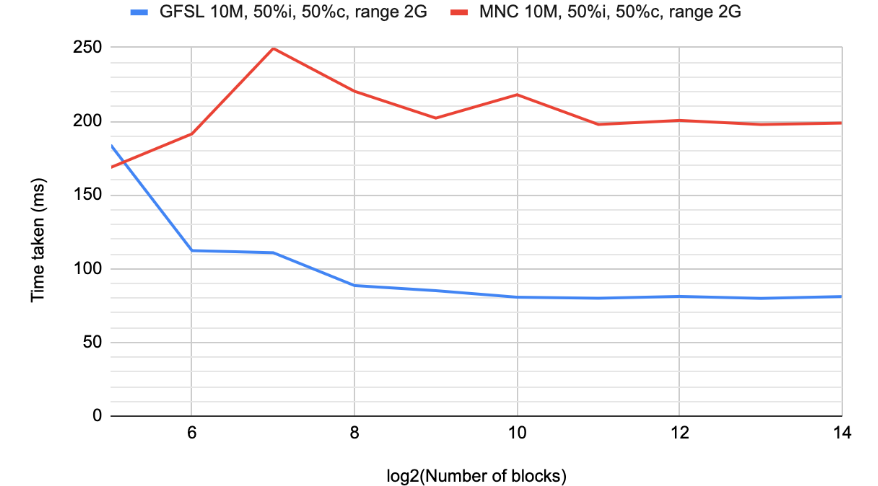
\includegraphics[width=0.8\textwidth]{5.png}
    \caption{Time taken(y-axis) vs. log2 (Number of blocks)(x-axis)}
\end{figure}

\subsubsection{10M Operations, 50\% Insert, 25\% erase, 50\% Search}
\begin{figure}[H]
    \centering
    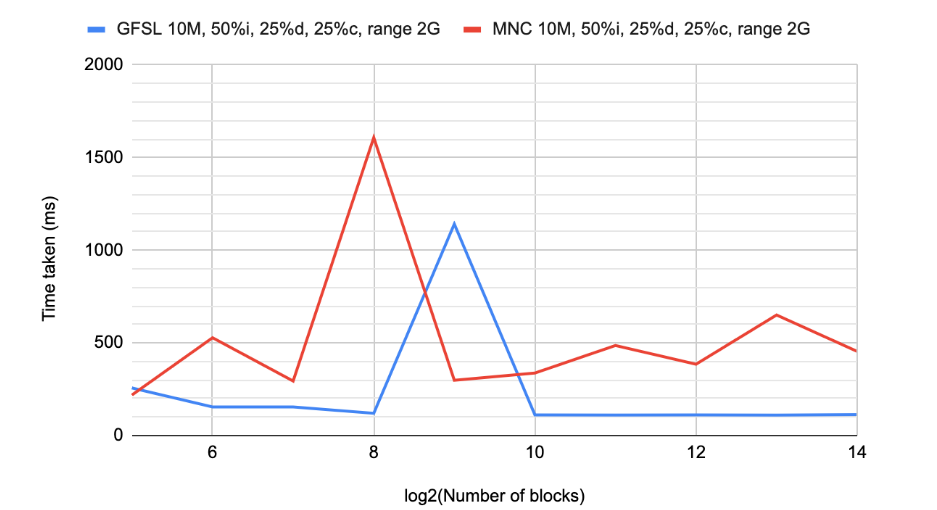
\includegraphics[width=0.8\textwidth]{6.png}
    \caption{Time taken(y-axis) vs. log2 (Number of blocks)(x-axis)}
\end{figure}

\subsubsection{100M Operations, 10\% Insert, 90\% Search}
\begin{figure}[H]
    \centering
    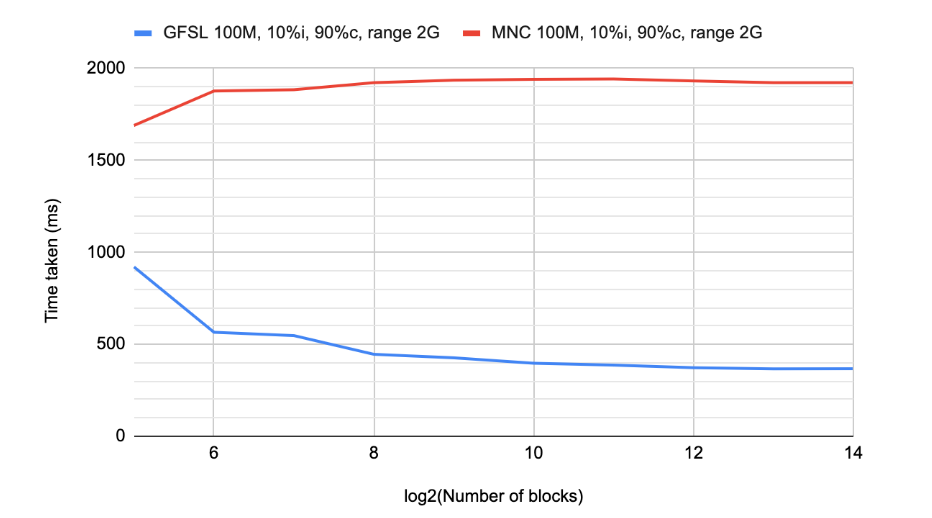
\includegraphics[width=0.8\textwidth]{7.png}
    \caption{Time taken(y-axis) vs. log2 (Number of blocks)(x-axis)}
\end{figure}

The most notable trend is that GFSL actually scales with the number of blocks, meanwhile M\&C actually starts to degrade after a certain number of blocks.

\subsection{Optimizations}

\subsubsection{Back-Off Locking}
Profiling the application shows that lock contention is a major bottleneck in GFSL, as contention on Chunks of higher level is very high. To mitigate this, we implement an exponential back-off algorithm, which improves performance by 10\%, in case of inserts and deletes.

\begin{figure}[H]
    \centering
    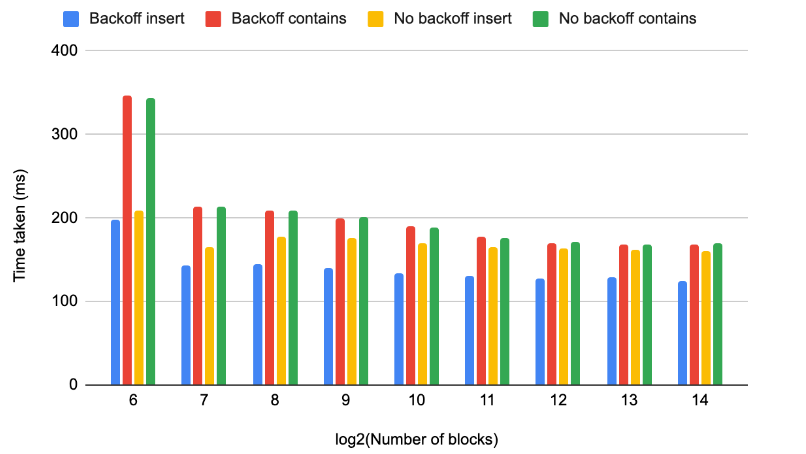
\includegraphics[width=0.8\textwidth]{8.png}
    \caption{Impact of exponential back off}
\end{figure}

\subsubsection{Keeping Chunks Unsorted}
In the original alogrithm, the chunks keys are always sorted. To maintain this property, insert and delete operations require sequential shifting of keys in the chunk atomically, which is a very expensive operation(on average 15 atomic writes for a single insertion or deletion). We remove this requirement by relaxing the sorting property of the Chunks. This requires the following changes-

\begin{itemize}
    \item In the search operation, to determine the next step from a Chunk, we now need to find the max of keys held by a subset of threads in a warp, this is the main tradeoff in this scheme.
    \item The shifting of keys in inserts and deletes is no longer needed, now we just find an empty slot and insert the key in just one atomic write.
    \item During the split operation, the greater half of the keys in a Chunk must be moved to the new chunk(to maintains the invariant that max key of a Chunk should only decrease), this was easy before since the Chunk was sorted. Now we need to find the median key using a Bitonic sort(implemented using warp shuffle intrinsics) before doing the split.
\end{itemize}


\begin{figure}[H]
    \centering
    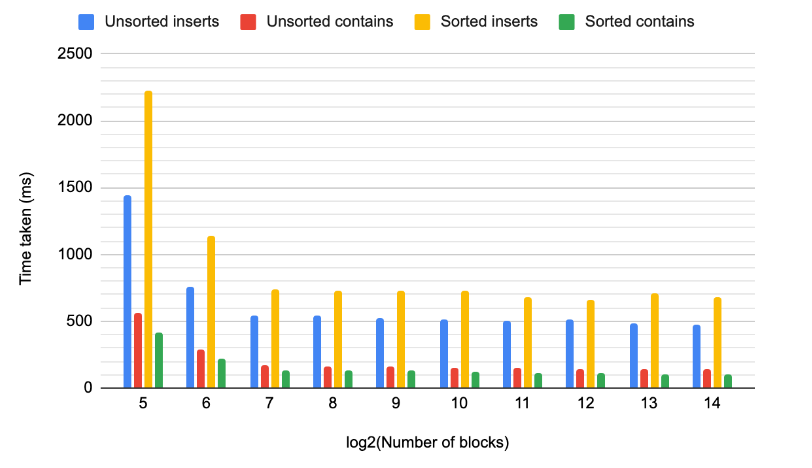
\includegraphics[width=0.8\textwidth]{9.png}
    \caption{Impact of Unsorted Chunks}
\end{figure}

We observe that on a workload contains more than 20\% write operations, the unsorted scheme outperforms the sorted scheme. The margin is more pronounced for higher write percentages.


% References
\bibliographystyle{plainnat}
\begin{thebibliography}{9}
\bibitem{herlihy2012art} 
Maurice Herlihy and Nir Shavit. 
\textit{The Art of Multiprocessor Programming}. 
Morgan Kaufmann, 2012.

\bibitem{mnc} 
Mishra, P. and Chaudhuri, M., 2012.
\textit{Performance Evaluation of Concurrent Lock-free Data Structures on GPUs}. 
ICPADS, 2012.

\bibitem{gfsl}
N. Moscovici, N. Cohen and E. Petrank.
\textit{A GPU-Friendly Skiplist Algorithm}. 
PACT, 2017

\end{thebibliography}

\end{document} 